\chapter{Pushdown Automater og Kontekstfrie Sprog}

Kontekstfrie Sprog er en klasse af sprog, som beskrives af hhv. Pushdown Automater og Kontekstfrie Grammatikker. Denne klasse af sprog er ``større'', det vil sige, indeholder flere mulige sprog end klassen af regulære sprog.

\section{Kontekstfrie Grammatikker}%
\label{sec:label}

\begin{definition}[Kontekstfri Grammatik]
	En kontekstfri grammatik er en 4-tuple $G = (V, \Sigma, R, S)$, hvor:
	\begin{itemize}
		\item $V$ er variablerne,
		\item $\Sigma$ er et endeligt alfabet,
		\item $R$ er substitueringsreglerne,
		\item $S$ er startsymbolet.
	\end{itemize}
\end{definition}

En \textit{afledning} $S \Rightarrow u_{1}A_{1}v_{1} \Rightarrow u_{2}A_{2}v_{2} \Rightarrow \cdots \Rightarrow u_{k}A_{k}v_{k} \Rightarrow w \in \Sigma^{*}$. Hvert skridt erstatter en variabel $A_{i}$ med højrehåndssiden af en regel i $R$. Vi skriver $S \stackrel{*}{\Rightarrow} w$ hvis $S$ kan aflede $w$ i en eller flere skridt. $L(G) = \{w \in \Sigma^{*} \mid S \stackrel{*}{\Rightarrow} w\}$.

Vi kalder denne sprogklasse \textit{kontekstfri}, da en erstatning af et symbol $A$ i f.eks. $uAv$ hvor $A \rightarrow \delta \in R$ ikke afhænger af $u$ af $v$, altså konteksten.

Uden at gå ind i detaljerne for hvad et parsetræ er, udover en grafisk forklaring på hvordan man afleder (eller udleder, jeg er ærligt i tvivl) en streng fra et symbol, kan man se et eksempel i Figur~\ref{fig:parsetreeg1} for følgende kontekstrfrie grammatik:

\begin{equation}
	\tag{$G_{1}$}
	\begin{split}
		A & \rightarrow \mathtt{0}A \mathtt{1} \\
		A & \rightarrow B                      \\
		B & \rightarrow \mathtt{\#}
	\end{split}
	\label{eqn:G1}
\end{equation}

\begin{figure}[ht]
	\centering
	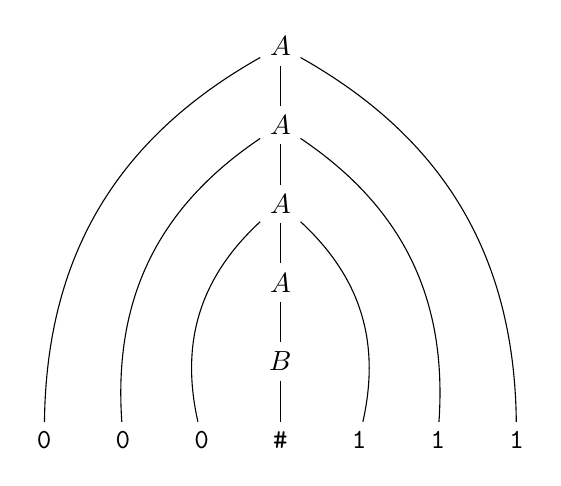
\begin{tikzpicture}[>=latex]
		% Nodes
		\node (0a) at (0,0) {\texttt{0}};
		\node (0b) at (1,0) {\texttt{0}};
		\node (0c) at (2,0) {\texttt{0}};
		\node (sharp) at (3,0) {\texttt{\#}};
		\node (1a) at (4,0) {\texttt{1}};
		\node (1b) at (5,0) {\texttt{1}};
		\node (1c) at (6,0) {\texttt{1}};

		% Upper nodes
		\node (B) at (3,1) {$B$};
		\node (A4) at (3,2) {$A$};
		\node (A3) at (3,3) {$A$};
		\node (A2) at (3,4) {$A$};
		\node (A1) at (3,5) {$A$};

		% Lines going down
		\draw[-] (B) to (sharp);
		\draw[-] (A4) to (B);
		\draw[-] (A3) to (A4);
		\draw[-] (A2) to (A3);
		\draw[-] (A1) to (A2);

		% Lines going to terminals
		\draw[-] (A1) to[bend right] (0a);
		\draw[-] (A1) to[bend left] (1c);
		\draw[-] (A2) to[bend right] (0b);
		\draw[-] (A2) to[bend left] (1b);
		\draw[-] (A3) to[bend right] (0c);
		\draw[-] (A3) to[bend left] (1a);

	\end{tikzpicture}
	\caption{\label{fig:parsetreeg1} Parse-træ for \texttt{000\#111} i \eqref{eqn:G1}}
\end{figure}


\subsection{Alle regulære sprog er kontekstfrie}%
\label{subsec:label}


\begin{theorem}
	Hvis $L$ er et regulært sprog, så er $L = L(G)$ for en kontekstfri grammatik $G$.
\end{theorem}
\begin{proof}
	Lad $M = (Q, \Sigma, \delta, q_0, F)$ være en DFA hvor $L(M) = L$. For alle tilstande $Q = \{q_{0}, \ldots, q_{k}\}$ lader vi hver tilstand være variabler i $G = (V, \Sigma, R, S)$, så $V = \{X_{0}, X_{1}, \ldots, X_{k}\}$. Reglerne i $G$ fungerer således:
	Hvis $\delta(q_{i}, a) = q_{j}$, så $X_{i} \rightarrow aX_{j} \in R$. Hvis $q_{\ell} \in F$ så $X_{\ell} \rightarrow \varepsilon \in R$. Ud fra denne definition er $X_{0}$ startsymbolet for $G$.
	Dermed, givet en DFA som følgende:

	\begin{center}
		\begin{tikzpicture}
			\node[state, initial] (q0) at (0,0) {$q_0$};
			\node[state, right of=q0] (qi1) {$q_{i_{1}}$};
			\node[state, right of=qi1] (qi2) {$q_{i_{2}}$};
			\node[state, accepting, right=4cm of qi2] (qn) {$q_{i_{n}}$};

			\draw  (q0) edge node{$a_{1}$} (qi1)
			(qi1) edge node{$a_{2}$} (qi2)
			(qi2) edge node{$\cdots, a_{n}$} (qn);

		\end{tikzpicture}
	\end{center}

	Får vi en afledning $X_{0} \Rightarrow a_{1}X_{i_{1}} \Rightarrow a_{1}a_{2} \ldots a_{n}X_{i_{n}} \Rightarrow a_{1}a_{2}\ldots a_{n} = w$
\end{proof}

\subsection{Kontrol af Medlemskab i et Kontekstfrit Sprog}%
\label{subsec:label}

Hvis vi vil vide om strengen $w$ accepteres af en DFA, finder vi bare ud af om DFA'en ``spiser'' den. Ved en NFA konverterer vi først til en DFA; hvilket kan give eksponentielle tilstande, men det er stadig ligeså simpelt.

Ved et kontekstfrit sprog er det ikke ligeså nemt. Faktisk er der ikke en måde at lave en øvre grænse på hvor lang tid det tager med en ``normal'' kontekstfri grammatik.

Vores løsning er at konvertere fra en ``normal'' kontekstfri grammatik, til en grammatik i det der kaldes \textit{Chomsky Normal Form}, eller hvad Jørgen kalder en ``Chomsky Grammar''. Dette sikrer at en afledning kan findes i $2|w|-1$ skridt, hvor $|w|$ er længden af strengen. I en Chomsky Grammatik har alle regler formen $A \rightarrow BC$ eller $A \rightarrow a$ og muligvis $S \rightarrow \varepsilon$ hvor $S$ er startsymbolet. Det er stadig lang tid, hvis der er 100 regler er det $100^{2|w|-1}$ mulige afledninger.

Vi får tallet $2|w|-1$ fra følgende argument: Den første afledning er af formen $S \rightarrow AB$ undtagen hvis $|w| = 1$. Du kan tænke på afledningen af strengen som først værende at finde variablerne der skal udlede (eller aflede, idk) til terminalerne, og så selve udledelsen til terminalerne. Fra den første afledningen $S \rightarrow AB$ er der $n-2$ (hvor $n = |w|$) skridt for at få de resterende variabler, og så er der $n$ afledningerne fra disse til variablerne. $ 1 + n-2 + n = 2n-1$.

\subsection{Chomsky Grammatik}%
\label{subsec:label}

\begin{theorem}
	Hvert kontekstfrit sprog er genereret af en kontekstfri grammatik i Chomsky Normal Form.
\end{theorem}

\begin{proof}
	Den ene retning er i sig selv korrekt, hvis $G$ er en Chomsky grammatik er det allerede en CFG. Den anden retning følger vi en algoritme:
	\begin{enumerate}
		\item Tilføj en ny startvariabel $S_{0}$
		\item Eleminér alle \(\varepsilon\)-regler ($A\rightarrow\varepsilon$) undtagen ved den nye startvariabel
		\item Eleminér alle $A \rightarrow B$ regler
		\item Konverter de lange regler $A \rightarrow A_{1}A_2 \ldots A_{n}$ hvor $n \ge 3$, til flere kortere regler, og konverter $A \rightarrow cd, A \rightarrow cD, A \rightarrow Cd$ til den rette format.
	\end{enumerate}

	Vi går i detaljer med hvert skridt:
	\begin{enumerate}
		\item Tilføj $S_{0}$ og reglen $S_{0} \rightarrow S$.
		      \begin{itemize}
			      \item Dermed kan startvariablen ikke være på højrehåndssiden af nogen regl. Det er klart her at $S \stackrel{*}{\Rightarrow} w \iff S_{0} \stackrel{*}{\Rightarrow} w$.
		      \end{itemize}
		\item Fjern $\varepsilon$-regler.
		      \begin{itemize}
			      \item Lav en ordning af variablerne i $V$
			      \item Gå hver variabel igennem efter denne ordning.
			      \item Hvis $A \rightarrow \varepsilon$ og $A$ er den næste variabel i ordnen med en $\varepsilon$ transition, så:
			      \item For hver regel $X \rightarrow \delta$ hvor $\delta$ kan være alt, men indeholder mindst én forekomst af $A$, så erstat hver delmængde med forekomsten af $A$ med et \(\varepsilon\).
			      \item For eksempel:
			            \begin{itemize}
				            \item $X \rightarrow uAvAw$ bliver til
				            \item $X \rightarrow uvw$
				            \item $X \rightarrow uAvw$
				            \item $X \rightarrow uvAw$
				            \item $X \rightarrow uAvAw$
			            \end{itemize}
			      \item Hvis $X \rightarrow A$ er en regel, så tilføj $X \rightarrow \varepsilon$, undtagen hvis du allerede har fjernet reglen $X \rightarrow \varepsilon$.
		      \end{itemize}
		\item Fjern ``unit regler''.
		      \begin{itemize}
			      \item Højrehåndssiden af en regel skal være af formen $AB$ eller $c$.
			      \item Hvis $A \rightarrow B$ er en regel, tilføj reglen $A \rightarrow u$ for alle $u$, hvor $B \rightarrow u$ i $R$, undtagen hvis denne allerede eksisterer.
			      \item Fortsæt dette indtil der ikke er flere unit regler.
		      \end{itemize}
		\item Fjern lange regler.
		      \begin{itemize}
			      \item Hvis $A \rightarrow u_{1}u_{2}, \ldots, u_{k}, k \ge 3 \; u_{i} \in V \cup \Sigma$ er en regel af $R$, så lav $k-2$ nye variabler $A_{1}, A_{2}, \ldots, A_{k-2}$ som kun gælder denne substitueringsregel.
			      \item Erstat $A \rightarrow \ldots$ med:
			            \begin{itemize}
				            \item $A \rightarrow u_{1}A_{1}$
				            \item $A_{1} \rightarrow u_{2}A_{2}$
				            \item $\vdots$
				            \item $A_{k-2} \rightarrow u_{k-}u_{k}$
			            \end{itemize}
			      \item Disse er dog ikke nødvendigvis lovlige, da en eller flere af $u_{i}$ kan være terminalsymboler.
			      \item Hvis $A \rightarrow u_{1}u_{2}$ er i $R$ med mindst en af $u_{1}, u_{2} \in \Sigma$ (altså er en terminal), så erstat denne $u_{i}$ med en ny variabel $U_{i}$ og lav reglen $U_{i} \rightarrow u_{i}$, for eksempel:
			            \begin{itemize}
				            \item $A \rightarrow bX$ erstattes af $A \rightarrow U_{b}X, U_{B} \rightarrow b$
			            \end{itemize}
		      \end{itemize}
	\end{enumerate}
\end{proof}

\section{Pushdown Automater}%
\label{sec:label}

En Pushdown Automat (PDA) minder om en NFA (men ikke en DFA!), dog med en stak tilsluttet til sig, hvilket giver den uendelige hukommelse. Man kan nemt med en PDA se hvordan den kan genkende det nonregulære sprog $\{a^{n}b^{n} \mid n \ge 0\}$:
\begin{itemize}
	\item Læs $a$'er, og for hvert læst, \textit{push} en til stakken.
	\item Læs $b$'er, og for hvert læst, \textit{pop} en fra stakken.
	\item Hvis stakken er tom og $w$ er læst, er strengen accepteret.
\end{itemize}

PDA'en i sig selv har ikke en måde at fortælle dig på, at stakken er tom eller ej. Her er en normal løsning at have et symbol udelukkende til at indikere at stakken er tom. Ofte bliver symbolet $\mathdollar $ brugt. Dermed, hvis PDA'en læser et $\mathdollar $ ved den at stakken er ``tom''. Et tilstandsdiagram af en PDA der genkender $\{0^{n}1^{n} \mid n \ge 0\}$ kan ses i Figur~\ref{fig:sipser2.15}.

\begin{figure}[ht]
	\centering
	\begin{tikzpicture}[>=Stealth,shorten >=1pt,node distance=2.8cm,on grid,auto]
		\node[state, accepting, initial] (q1) {$q_1$};
		\node[state, right=of q1] (q2) {$q_2$};
		\node[state, below=of q2] (q3) {$q_3$};
		\node[state, accepting, left=of q3] (q4) {$q_4$};

		\path[->]
		(q1) edge node {$\varepsilon, \varepsilon \rightarrow \$$} (q2)
		(q2) edge[loop right] node {$0, \varepsilon \rightarrow 0$} (q2)
		(q2) edge node {$1, 0 \rightarrow \varepsilon$} (q3)
		(q3) edge[loop right] node {$1, 0 \rightarrow \varepsilon$} (q3)
		(q3) edge node { $\varepsilon, \$ \rightarrow \varepsilon$ } (q4);
	\end{tikzpicture}
	\caption{\label{fig:sipser2.15} State diagram af PDA'en $M_1, L(M_1) = \{0^n 1^n  | n \ge 0 \}$}
\end{figure}

Bemærk fra tilstandsdiagrammet at $\varepsilon \rightarrow a$ betyder at symbolet $a$ bliver \textit{pushet} til stakken, og $a \rightarrow \varepsilon$ betyder at $a$ bliver \textit{poppet}.


\begin{definition}[Formel Definition af en Pushdown Automat]
	\label{def:pda}
	En \textit{pushdown automat} er en 6-tuple $(Q, \Sigma, \Gamma, \delta, q_{0}, F)$, hvor $Q$, $\Sigma$, $\Gamma$, og $F$ alle er endelige sæt, og
	\begin{enumerate}
		\item $Q$ er sættet af states
		\item $\Sigma$ er input alfabetet
		\item $\Gamma$ er stak alfabetet
		\item $\delta : Q \times \Sigma_{\varepsilon} \times \Gamma_{\varepsilon} \longrightarrow P(Q \times \Gamma_{\varepsilon})$ er overføringsfunktionen
		\item $q_{0} \in Q$ er start staten
		\item $F \subseteq Q$ er sættet af accept states.
	\end{enumerate}
\end{definition}

\section{Ækvivalens mellem PDA og CFG}%
\label{sec:label}

\begin{theorem}
	Et sprog $L$ er kontekstfrit $\iff$ $L$ accepteres af en PDA $M$.
\end{theorem}
Vi deler det op i to beviser, et der beviser ``Et sprog $L$ er kontekstfrit \(\Rightarrow\) $L$ accepteres af en PDA $M$'', og derefter omvendt.

\begin{proof}[Et sprog $L$ er kontekstfrit \(\Rightarrow\) $L$ accepteres af en PDA $M$]
	Måden vi beviser dette på, er ved at bygge en PDA der ``efterligner'' en kontekstfri grammatik.
	\begin{definition}[Venstremest afledning]
		En venstremest afledning er en afledning der altid tager det venstremeste symbol i en regel.
	\end{definition}
	Vi antager at $G$ er en Chomsky Grammatik. Hvis ikke, kan vi konvertere den inden.

	Vi laver en algoritme der fungerer som følger:
	\begin{itemize}
		\item Først putter vi $\mathdollar$ på stakken og $S$ over, hvor $S$ er startsymbolet af $G$.
		\item Gentag:
		      \begin{itemize}
			      \item Hvis symbolet på toppen af stakken er en variabel, så nondeterministisk vælg en regel $A \rightarrow \beta \in R$ og erstat $A$ på stakken med $\beta$, som, da det er en Chomsky Grammatik enten af $A_{1}A_{2}$ eller $a \in \Sigma$. Bemærk at vi pusher variabler på en sådan måde at den venstremest variabel er øverst på stakken.
			      \item Hvis toppen af stakken er en $a \in \Sigma$, altså en terminal, så læs det næste inputsymbol $a'$. Hvis $a' = a$, så fjern $a$ fra stakken. Ellers, \textit{afvis} denne gren.
			      \item Hvis toppen af stakken er $\mathdollar$, så gå til \textit{accept} tilstanden.
		      \end{itemize}
	\end{itemize}

	Vi laver en notation $a, A \rightarrow A_{1}A_{2}$ der siger at når $a$ læses, så pop $A$ og push $A_{1}A_{2}$. Vi kan simpelt implementere dette, ved at lave en mellem-tilstand, hvor overføringen fra den originale til denne mellem har $a, A \rightarrow A_{2}$ og overføringen fra denne mellem til ``slut''tilstanden har overføringen $\varepsilon, \varepsilon \rightarrow A_{1}$. Altså er mellemtilstanden udelukkende brugt for overføringen.

	Vi kan nu se et tilstandsdiagram der viser hvordan denne PDA vil fungere (bemærk dog at den vil være anderledes for hver CFG):

	\begin{center}
		\begin{tikzpicture}[shorten >=1pt, node distance=2.0cm, on grid, auto]
			\node[state, initial] (q1) {$q_{\text{start}}$};
			\node[state, below=of q1] (q2) {$q_{\text{loop}}$};
			\node[state, accepting, below=of q2] (q3) {$q_{\text{accept}}$};

			\path[->]
			(q1) edge node {$\varepsilon, \varepsilon \rightarrow S \mathdollar$} (q2)
			(q2) edge[loop right] node[align=center] {$\varepsilon, A \rightarrow w \; \; \text{ for reglen }A \rightarrow w$\\$a, a \rightarrow \varepsilon \; \;  \text{for terminalen } a$} (q2)
			(q2) edge node {$\varepsilon, \mathdollar \rightarrow \varepsilon$} (q3);
		\end{tikzpicture}
	\end{center}
\end{proof}

\begin{proof}[Et sprog $L = L(M)$ for en PDA $\Rightarrow$ $L = L(G)$ for kontekstfri grammatik $G$]
	Dette bevis er en del mere kompliceret end det andet.\\
	\noindent
	\textit{Skridt 1}:\\
	Vi definerer nu en meget begrænset PDA med følgende betingelser:
	\begin{enumerate}
		\item Der er kun én accepttilstand.
		\item Stakken tømmes \textit{altid} før en streng accepteres.
		\item Hvor overføring popper enten et symbol eller pusher det.
	\end{enumerate}

	Den første betingelse kan simpelt implementeres, ved at fjerne \textit{accept} fra alle tidligere accept states, og give \(\varepsilon\)-overføringer til den nye.
	Den anden betingelse er også simpel. Vi kan lave en mellemtilstand der kommer ind før accepttilstanden, som popper alle symboler indtil stakken er tom. Den tredje betingelse er også simpel, men kræver lidt mere. Ved en overføring der både popper og pusher skal vi ændre det til at være to overføringer med en mellemtilstand, hvor der først poppes til mellemtilstanden, og derefter pushes til den originale ``slut''tilstand. Hvis der ikke poppes eller pushes gør vi det samme, men hvor vi først pusher et ligegyldigt symbol, som vi så popper igen med det samme bagefter.\\\\
	\noindent
	\textit{Skridt 2}:\\
	Her vil vi forstå hvordan en PDA $M$ ændrer på sin stak imens den gennemgår en streng $w$.

	Hvis vi går fra en tilstand $p$ hvor stakken er udelukkende symbolet til at indikere slutningen på stakken, $\mathdollar$, til en tilstand $q$ også udelukkende med $\mathdollar$, så, grundet vores antagelse at stakken kun tømmes fudlstændig før en streng accepteres, kan vi antage at der muligvis bliver pushet ting til stakken, men der bliver ikke poppet under.

	Ved en sådan walk, kan vi også antage at hvis vi er på et niveau \(\ell\), så vil en walk fra $p$ til $q$ ikke poppe nogen symboler under niveau \(\ell\).\\\\
	\textit{Skridt 3}\\
	\noindent
	For alle valgene af tilstande $p, q \in Q(M)$ vil $G$ indeholde en variabel $A_{pq}$. $A_{pq}$ vil generere alle strenge $w \in \Sigma^{*}$ på samme måde som ved skridt 2, altså hvor vi starter med en stak på niveau \(\ell\) og slutter med en stak på niveau \(\ell\); uden at stakken er blevet poppet til under niveau \(\ell\).

	Der er nu to muligheder til når $M$ spiser $w$ og går fra tilstand $p$ på et stkaniveau $\ell$ til en tilstand $q$ på et stakniveau \(\ell\), og aldrig går under niveau \(\ell\) på stakken:
	\begin{enumerate}
		\item[a)] $M$'s stak er på niveau \(\ell\) til at starte med, og efter at have læst $w$, men imellem er den over \(\ell\).
		\item[b)] After at have læst en del af $w$ er stakken tilbage nede på niveau \(\ell\) og går op igen før hele $w$ bliver læst.
	\end{enumerate}

	I tilfælde $b)$ kan vi opdele grammatikken til to eller flere, hvor de ``stopper'' når $M$ ryger ned på niveau \(\ell\) igen. Hvis vi kalder dennet tilstand $r$, så kan vi sige at når vi går fra tilstand $p$ til $r$ afleder den strengen $u$; og når den går fra $r$ til $q$ genererer den $v$. Så akn vi skrive $w = uv$ og $A_{pr} \stackrel{*}{\Rightarrow} u$ og $A_{rq} \stackrel{*}{\Rightarrow} v$.

	Vi definerer nu grammatikken ud fra disse muligheder. Husk at en grammatik $G$ er en 4-tuple $(V, \Sigma, R, S)$.
	\begin{itemize}
		\item $V = \{A_{pq} \mid p, q \in Q(M)\}$. Det vil sige at hvis $M$ er antallet af tilstande, så er der $M^{2}$ symboler.
		\item $S = A_{q_{0}, q_{\text{accept}}}$
		\item Regler:
		      \begin{itemize}
			      \item $\forall p,q,r,s \in Q(M) \; \forall t \in \Gamma \; \forall a,b \in \Sigma_{\varepsilon}$:
			            \begin{itemize}

				            \item Hvis PDA'en har to overføringer:
				                  \begin{itemize}
					                  \item Fra $p$ til $r$ på overføring der læser $a$ og pusher $t$
					                  \item Fra $s$ til $q$ på en overføring der læser $b$ og popper $t$
				                  \end{itemize}
				            \item Så tilføj $A_{pq} \rightarrow aA_{rs}b$ til $R$.
			            \end{itemize}
			      \item \(\forall p, q, r \in Q(M)\) tilføj $A_{pq} \rightarrow A_{pr}A_{rq}$ til $R$
			      \item \(\forall p \in Q\) tilføj $A_{pp} \rightarrow \varepsilon$ til $R$.
		      \end{itemize}
	\end{itemize}

	Vi går nu videre til delen, hvor vi vil bevise at alt som PDA'en vi har konverteret til en CFG kan acceptere, vil vores CFG også acceptere, og hvis den afviser, vil vi også afvise.

	\begin{claim}
		$A_{pq} \stackrel{*}{\Rightarrow} x \Rightarrow$ at vi kan gå fra $p$ til $q$ uden at gå under niveau \(\ell\).
	\end{claim}
	\begin{proof}
		Vi beviser ved induktion over antallet af skridt i afledningen.

		Et skridt: $p = q$ og $A_{pp} \rightarrow \varepsilon$ da $x \in \Sigma^{*}$. Her er det tydeligt at $m$ kan gå fra niveau \(\ell\) til niveau \(\ell\) uden at røre ved stakken overhovedet.

		Hypoteses: Sandt når der er mindre end eller lig med $k$ skridt i afledningen.

		Vi kigger på en afldening med $k+1$ skridt og kigger på den første regel brugt i afledningen. Hvis $A_{pq} \rightarrow aA_{rs}b$ så $x = ayb$ hvor $A_{rs} \stackrel{*}{\Rightarrow} y$. Denne har $k$ skridt, så ved induktion må der ikke laves noget på stakken. Dermed vil $a$ pushe noget og $b$ poppe.

	\end{proof}
\end{proof}




%%% Local Variables:
%%% mode: latex
%%% TeX-engine: xetex
%%% TeX-command-extra-options: "-shell-escape"
%%% TeX-master: "main"
%%% End:
